\documentclass{article}
\usepackage{geometry}
\geometry{a4paper, margin=1in}
\usepackage{tikz}
\usetikzlibrary{shapes.geometric, arrows.meta, positioning}
\usepackage{enumitem}
\usepackage{amsmath}
\usepackage{hyperref}

\title{Key Concepts and Theory Behind LangGraph for Multi-Agent Systems}
\author{Grok, created by xAI}
\date{\today}

\begin{document}

\maketitle

\section{Introduction}

LangGraph is an open-source framework developed by the creators of LangChain to facilitate the design, orchestration, and deployment of stateful, multi-agent applications powered by large language models (LLMs). Unlike traditional linear workflows, LangGraph leverages graph-based architectures to model complex interactions among multiple agents, enabling dynamic, cyclical, and context-aware workflows. This document provides a comprehensive introduction to LangGraph, detailing its theoretical foundations, key concepts, organizational logic, and practical implementation for building multi-agent systems. Through diagrams and explanations, we aim to elucidate how LangGraph structures agent interactions and how its components are utilized to create robust AI systems.

\section{What is LangGraph?}

LangGraph is a low-level orchestration framework built on top of LangChain, designed to create controllable and scalable multi-agent systems. It extends LangChain’s capabilities by introducing graph-based workflows, where nodes represent agents or tasks, and edges define the flow of information or control between them. This graph-based approach supports cyclical interactions, state persistence, and human-in-the-loop (HITL) integrations, making it ideal for applications requiring complex reasoning, collaboration, and context retention, such as autonomous assistants, research systems, or debate simulations.

LangGraph’s primary goal is to provide developers with fine-grained control over agent workflows without imposing rigid abstractions. It achieves this through a stateful design, where a shared state object tracks the system’s progress, enabling memory, error recovery, and dynamic decision-making. By modeling workflows as directed graphs, LangGraph supports both deterministic and dynamic control flows, allowing agents to adapt to evolving contexts and user inputs.

\section{Theoretical Foundations}

LangGraph is grounded in several theoretical concepts that underpin its design and functionality:

\begin{itemize}
    \item \textbf{Graph Theory:} LangGraph represents workflows as directed graphs, with nodes (agents or tasks) and edges (information or control flow). This structure supports both acyclic (DAGs) and cyclic graphs, enabling loops for iterative reasoning or task refinement.
    \item \textbf{State Machines:} LangGraph conceptualizes workflows as state machines, where each state represents a point in the workflow (e.g., an agent’s action or a decision point), and transitions are governed by conditions or agent outputs. This allows for structured yet flexible control flows.
    \item \textbf{Agent-Based Modeling:} Multi-agent systems in LangGraph simulate environments where autonomous agents collaborate or compete to achieve goals. Each agent operates with specific roles, tools, or objectives, interacting through a shared state.
    \item \textbf{Natural Language Processing (NLP):} LangGraph leverages LLMs for agent reasoning, tool calling, and state updates, relying on NLP to process inputs, generate responses, and evaluate outputs.
    \item \textbf{Control Theory:} The framework incorporates feedback loops (e.g., HITL, checkpoints) to ensure reliability, allowing the system to adapt based on external inputs or internal evaluations.
\end{itemize}

\section{Key Concepts in LangGraph}

To understand how LangGraph operates, the following key concepts are essential:

\begin{itemize}
    \item \textbf{Nodes:} Nodes represent units of work, such as an agent’s action, a tool call, or a decision point. Each node is typically a Python function that processes the current state and returns updates or outputs.
    \item \textbf{Edges:} Edges define the flow of control or data between nodes. They can be normal (deterministic transitions) or conditional (based on state or agent decisions), enabling dynamic routing.
    \item \textbf{State:} The state is a shared data structure (e.g., a dictionary or typed class) that persists across the workflow, tracking information like messages, agent outputs, or internal variables. It ensures context retention and supports memory.
    \item \textbf{Checkpointers:} Checkpointers provide persistence by saving the state at each step, enabling features like time travel (replaying past states), error recovery, and HITL interactions.
    \item \textbf{Human-in-the-Loop (HITL):} LangGraph supports pausing execution to incorporate human feedback, allowing for validation, correction, or steering of agent actions.
    \item \textbf{Memory:} Memory enables agents to recall past interactions or states, implemented through the state object and checkpointers. It supports both short-term (session-based) and long-term (persistent) memory.
    \item \textbf{Streaming:} LangGraph provides token-by-token streaming and intermediate step streaming, allowing real-time visibility into agent reasoning and actions.
    \item \textbf{Subgraphs:} Complex workflows can be modularized into subgraphs, where a node itself is a graph. Subgraphs enable hierarchical or specialized agent teams with their own state schemas.
\end{itemize}

\section{Organizational Logic of LangGraph}

LangGraph organizes multi-agent systems as directed graphs, where the workflow’s logic is defined by the structure of nodes and edges. The system operates as follows:

\begin{enumerate}
    \item \textbf{Initialization:} A \texttt{StateGraph} is created with a state schema (e.g., a \texttt{TypedDict} defining keys like \texttt{messages} or \texttt{agent\_outcome}). This schema dictates what information is tracked.
    \item \textbf{Node Definition:} Nodes are added to the graph, each corresponding to an agent, tool, or router function. For example, a debate agent node generates comments, while a referee node evaluates them.
    \item \textbf{Edge Configuration:} Edges are defined to specify transitions between nodes. Normal edges follow a fixed sequence, while conditional edges use a router function to decide the next node based on the state (e.g., a supervisor agent’s decision).
    \item \textbf{State Updates:} Each node processes the current state and returns updates, which are applied to the shared state using operators (e.g., appending messages). Checkpointers save the state for persistence.
    \item \textbf{Execution:} The graph is compiled and invoked with an initial input. The system traverses nodes according to edges, updating the state until a terminal condition (e.g., an \texttt{END} node) is reached.
\end{enumerate}

This logic enables LangGraph to support diverse control flows, such as sequential (one agent after another), hierarchical (supervisor-subordinate), or dynamic (LLM-driven routing). The state machine paradigm ensures that the system remains deterministic when needed while allowing flexibility for adaptive behaviors.

\section{Multi-Agent System Organization}

In a LangGraph-based multi-agent system, agents are organized as nodes within a graph, interacting through a shared state. Below is a typical structure for a debate system, as an example:

\begin{itemize}
    \item \textbf{Debate Agents:} Each agent is a node responsible for generating comments based on the topic and prior messages. Agents may have distinct roles (e.g., proponent, opponent) and use LLMs to produce responses.
    \item \textbf{Supervisor Agent:} A supervisor node (e.g., a router) decides which agent acts next or whether to end the conversation. It uses conditional edges to route based on state conditions, such as turn counts or content analysis.
    \item \textbf{Referee Agent:} A specialized node evaluates agent outputs using an LLM, assessing metrics like ethical soundness or relevance. The referee updates the state with evaluation results.
    \item \textbf{Tools:} Agents may call external tools (e.g., web search, database queries) as nodes, with outputs fed back into the state for further processing.
\end{itemize}

The shared state ensures all agents have access to the conversation history, evaluation results, and other context. Checkpointers persist this state, allowing the system to resume from interruptions or rewind for debugging.

\subsection{Diagram: Multi-Agent Debate System}

The following diagram illustrates a LangGraph-based debate system with multiple agents, a supervisor, and a referee:

\begin{figure}[h]
\centering
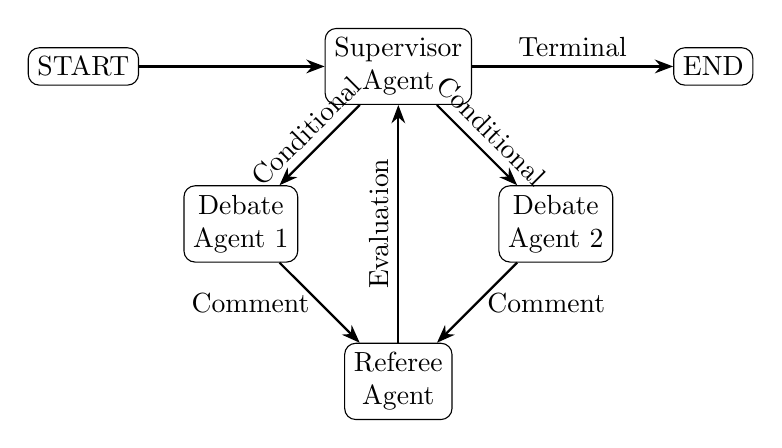
\begin{tikzpicture}[
    node/.style={rectangle, draw, rounded corners, minimum height=1em, minimum width=2em, align=center},
    arrow/.style={-Stealth, thick},
    ]
    % Nodes
    \node[node] (start) at (0,0) {START};
    \node[node] (supervisor) at (4,0) {Supervisor\\Agent};
    \node[node] (agent1) at (2,-2) {Debate\\Agent 1};
    \node[node] (agent2) at (6,-2) {Debate\\Agent 2};
    \node[node] (referee) at (4,-4) {Referee\\Agent};
    \node[node] (end) at (8,0) {END};

    % Edges
    \draw[arrow] (start) -- (supervisor);
    \draw[arrow] (supervisor) -- node[above, sloped] {Conditional} (agent1);
    \draw[arrow] (supervisor) -- node[above, sloped] {Conditional} (agent2);
    \draw[arrow] (agent1) -- node[left] {Comment} (referee);
    \draw[arrow] (agent2) -- node[right] {Comment} (referee);
    \draw[arrow] (referee) -- node[above, sloped] {Evaluation} (supervisor);
    \draw[arrow] (supervisor) -- node[above] {Terminal} (end);
\end{tikzpicture}
\caption{LangGraph multi-agent debate system with supervisor and referee agents.}
\end{figure}

In this diagram:
- The \texttt{START} node initializes the state with the debate topic.
- The \texttt{Supervisor Agent} routes to \texttt{Debate Agent 1} or \texttt{Debate Agent 2} based on state conditions (e.g., turn order).
- Debate agents generate comments, which are evaluated by the \texttt{Referee Agent}.
- The referee’s evaluation updates the state, and the supervisor decides whether to continue or terminate at the \texttt{END} node.

\section{Creating a Multi-Agent System with LangGraph}

Building a multi-agent system in LangGraph involves the following steps, aligned with the key concepts:

\begin{enumerate}
    \item \textbf{Define the State Schema:} Create a \texttt{TypedDict} or class to define the state structure. For a debate system, this might include:
    \begin{verbatim}
from typing import TypedDict, List
from langchain_core.messages import BaseMessage
class DebateState(TypedDict):
    topic: str
    messages: List[BaseMessage]
    evaluations: List[dict]
    turn_count: int
    \end{verbatim}

    \item \textbf{Implement Agent Nodes:} Define functions for each agent. For example, a debate agent generates comments using an LLM, while the referee evaluates them:
    \begin{verbatim}
def debate_agent(state: DebateState) -> DebateState:
    llm = ChatOpenAI(model="gpt-4o")
    prompt = f"Topic: {state['topic']}\nHistory: {state['messages']}"
    response = llm.invoke(prompt)
    return {"messages": state["messages"] + [response]}

def referee_agent(state: DebateState) -> DebateState:
    llm = ChatOpenAI(model="gpt-4o")
    comment = state["messages"][-1].content
    evaluation = llm.invoke(f"Evaluate: {comment}")
    return {"evaluations": state["evaluations"] + [evaluation]}
    \end{verbatim}

    \item \textbf{Configure the Graph:} Use \texttt{StateGraph} to add nodes and edges:
    \begin{verbatim}
from langgraph.graph import StateGraph, START, END
graph = StateGraph(DebateState)
graph.add_node("debate_agent_1", debate_agent)
graph.add_node("debate_agent_2", debate_agent)
graph.add_node("referee", referee_agent)
graph.add_node("supervisor", supervisor)
graph.add_edge(START, "supervisor")
graph.add_conditional_edges("supervisor", route_agents)
graph.add_edge("debate_agent_1", "referee")
graph.add_edge("debate_agent_2", "referee")
graph.add_edge("referee", "supervisor")
graph.add_conditional_edges("supervisor", end_condition, {END: END})
    \end{verbatim}

    \item \textbf{Compile and Run:} Compile the graph and invoke it with an initial state:
    \begin{verbatim}
compiled_graph = graph.compile(checkpointer=MemorySaver())
result = compiled_graph.invoke({"topic": "AI ethics", "messages": [],
                               "evaluations": [], "turn_count": 0})
    \end{verbatim}
\end{enumerate}

\section{Code Structure and Implementation}

The LangGraph implementation relies on the LangChain ecosystem, particularly \texttt{langchain-core} and \texttt{langchain-openai} for LLM interactions. Key components include:

\begin{itemize}
    \item \texttt{StateGraph:} The core class for defining the graph structure, nodes, and edges.
    \item \texttt{Checkpointers:} Classes like \texttt{MemorySaver} for state persistence.
    \item \texttt{ToolNode:} A prebuilt node for executing external tools (e.g., web search).
    \item \texttt{ChatOpenAI:} An LLM wrapper for generating agent responses or evaluations.
\end{itemize}

The \texttt{build\_debate\_graph} function (hypothetical in this context) constructs the graph by defining nodes for debate agents, a supervisor, and a referee, with edges governing their interactions. The \texttt{RefereeAgent} class processes comments using an LLM, formats evaluation prompts, and returns structured outputs (e.g., ethical scores, sentiment).

\section{Conclusion}

LangGraph provides a powerful framework for building stateful, multi-agent systems, leveraging graph-based workflows to orchestrate complex interactions. Its key concepts—nodes, edges, state, checkpointers, and memory—enable developers to create flexible, controllable, and context-aware applications. By organizing agents as nodes in a graph and using a shared state for communication, LangGraph supports dynamic collaboration, as illustrated in the debate system example. The provided diagrams and code snippets demonstrate how to structure and implement such systems, offering a foundation for further exploration and expertise in agent-based AI development.

For further learning, explore the LangChain Academy’s LangGraph course or the official documentation at \url{https://langchain-ai.github.io/langgraph/}.

\end{document}
